
\chapter{Experimental Evaluation}

In this chapter it will be discussed the function's effective performance and examine the accuracy and effectiveness of the queries. To compare the offline and online executions, we will also balance the differences between it in real time with the C implementation handling the same data.

\section{Performance}
This section will analyze and discuss the performance of the sql function by varying the lambda parameter and the number of points.
\begin{table}[htbp]
    \centering
    \label{tab:execution_time}
    \begin{tabular}{@{}lccccc@{}}
        \toprule
        Number of Points & \multicolumn{5}{c}{Lambda} \\
        \cmidrule{2-6}
        & 1         & 0.75       & 0.5        & 0.25       & 0.01       \\
        \midrule
        100              & 00.001137 & 00.001965 & 00.002775 & 00.003328 & 00.004529 \\
        1000             & 00.01498  & 00.014966 & 00.022183 & 00.024588 & 00.023035 \\
        10000            & 00.164196 & 00.215692 & 00.214011 & 00.247379 & 00.218447 \\
        100000           & 01.77365  & 02.171435 & 02.844324 & 02.617976 & 02.437037 \\
        1000000          & 04.618455 & 05.371317 & 06.461961 & 06.021071 & 04.510934 \\
        \bottomrule
    \end{tabular}
    \caption{Average Execution Time by Number of Points and Lambda}
\end{table}

In order to get those results we benchmark the request 10 times for each requests and retrieve the average of those executions. As standalone results it has no real meaning outside but we can notice that the speed of the algorithm increase around $0.5$ and decrease outside those values of lambda. We can also state that maybe there is another value as maximum execution time between $0.75$ and $0.25$ . We can state that this is maybe because the number of instruction that mix setting in a priority queue and the instructions of reduction is around $0.5$. Because when lambda is equal to 1 there is no reduction and only setting in the maximal size of a priority queue and adjust priority operation and when lambda go towards $0$ there is a lot of reduction operation and setting in the minimal size of a priority queue. That is an explanation that could befit those data. When the size of the input is multiplying by $10$ the execution time is around $2$ times longer.

\subsection{Comparison with C}
In order to have meaning to those result we will compare it with the C implementation using the real time approach and to see between the offline and the online approach the difference that happen.

\begin{table}[htbp]
    \centering
    \label{tab:execution_time_c}
    \begin{tabular}{@{}lccccc@{}}
        \toprule
        Number of Points & \multicolumn{5}{c}{Lambda} \\
        \cmidrule{2-6}
        & 1         & 0.75       & 0.5        & 0.25       & 0.01       \\
        \midrule
        100              & 00.000094 & 00.000092 & 00.00009 & 00.000098 & 00.000096 \\
        1000             & 00.00081  & 00.000822 & 00.000943 & 00.000876 & 00.000788 \\
        10000            & 00.008889 & 00.008852 & 00.008663 & 00.008263 & 00.00818 \\
        100000           & 00.090018  & 00.088485 & 00.089533 & 00.089064 & 00.088728 \\
        1000000          & 00.892172 & 00.864116 & 00.870661 & 00.937186 & 00.920517 \\
        \bottomrule
    \end{tabular}
    \caption{Average Execution Time (C) by Number of Points and Lambda}
\end{table}

As we can see, executing C code is much faster than executing sql queries, which makes execution and simplification using steam processing techniques in C both viable and possible. The speed is such that even for 1 million points the average execution time is less than 1 second.

\section{Precision}
This section will focus on the precision of the simplification using the same parameter as before in order to have an idea of the quality of the simplification in a function of lambda and types of path. We will discuss on trajectory based on AIS dataset. As stated in \cite{abam2007streaming}, there is different type of path as convex and concave. As a reminder this work focus on the simplification of lines and do not take into account land or see restriction during the simplification process. In this section we will analyze different trajectory defines them and see with different lambda and metrics evaluation the quality of the simplification. At the end we will run in a big datasets and see the results as a graph and discuss them.

\subsection{Trajectory 1}

\begin{figure}[!h]
    \centering
    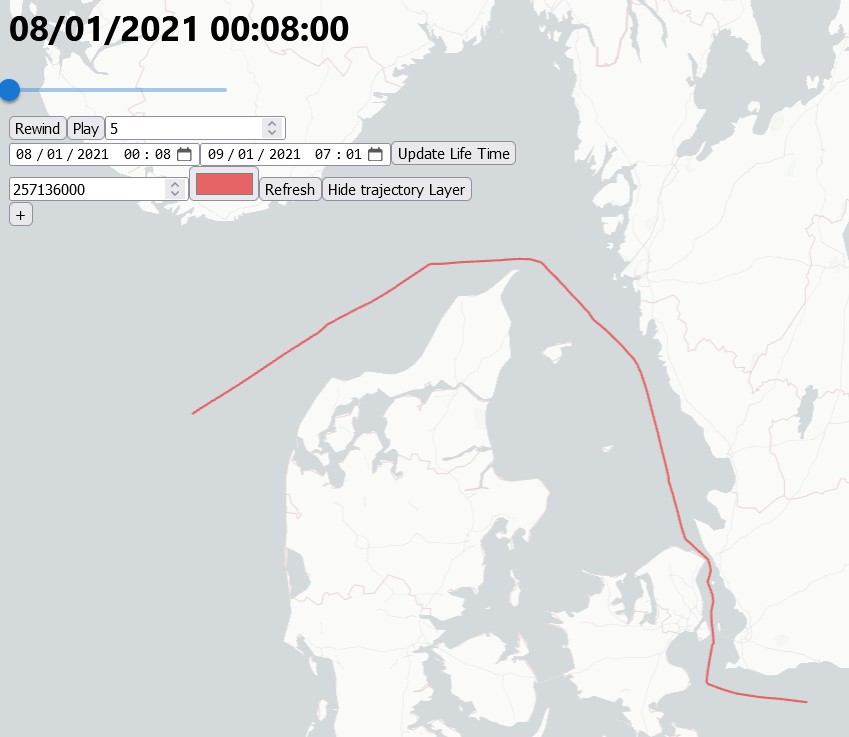
\includegraphics[width=0.5\linewidth]{figures/Stats/traj_1.jpg}
    \caption{Trajectory 1}
    \label{fig:traj_1}
\end{figure}

This trajectory is composed of 20865 points and begin at 1am the 8/1/2021 with a duration of 1 day. This trajectory have convex and concave path in order to analyze the effect of the simplification in those specific moment. The precision of the trajectory will be computed based on the current metrics proposed in the state of the art such as Frechet distance and Hausdorff distances. We will not discuss the precision of lambda 1 because it does not reduce any points from the original trajectory.



\begin{figure}[!h]
    \centering
    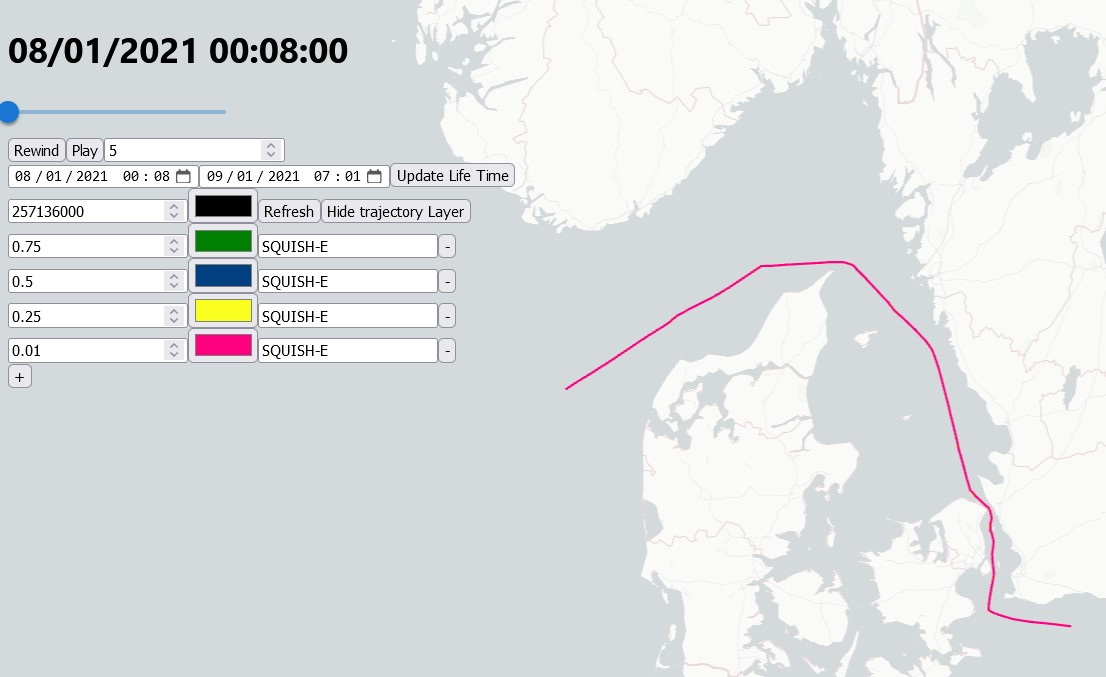
\includegraphics[width=0.5\linewidth]{figures/Stats/squish_1.jpg}
    \caption{Trajectory 1 - SQUISH-E}
    \label{fig:traj_1_squish}
\end{figure}

The path looks really similar and is close to the original path in \ref{fig:traj_1_squish}. In order to see the differences we can zoom and move the slider in order to see the moving objects in relation with the current time.

\begin{figure}[!h]
    \centering
    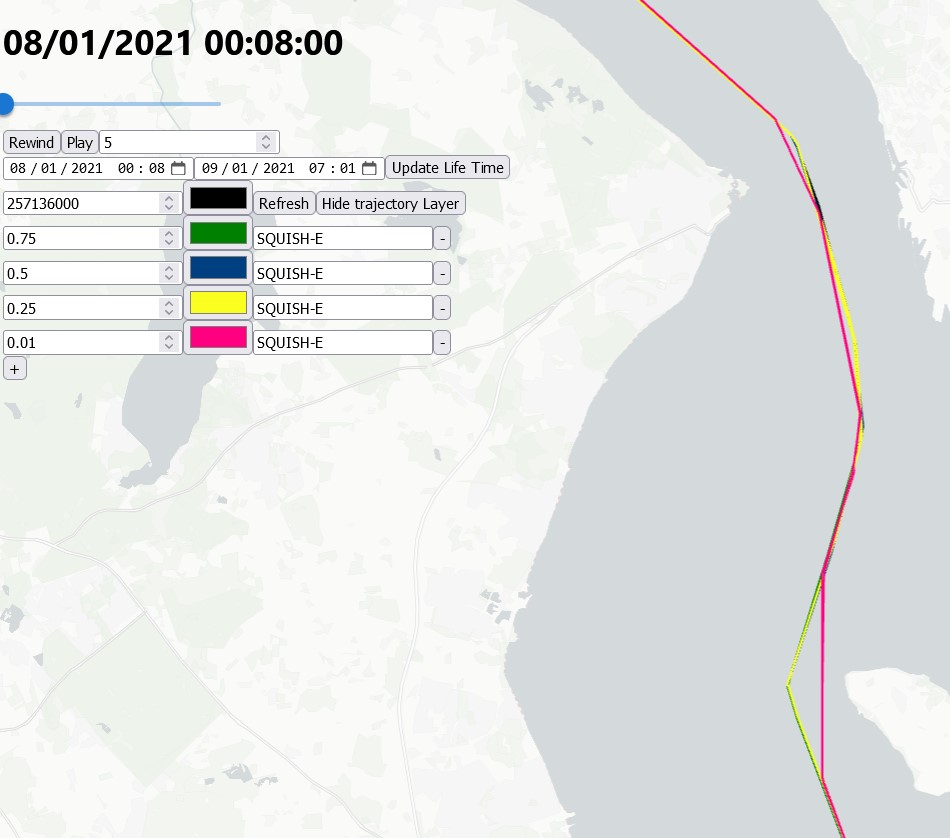
\includegraphics[width=0.5\linewidth]{figures/Stats/squish_1_zoom.jpg}
    \caption{Trajectory 1 - ZOOM }
    \label{fig:traj_1_sqzoom}
\end{figure}

In this we can see the path being simplified where there is curves and having less precision as lambda decreases.

\begin{table}[htbp]
    \centering
    \label{tab:precision_metrics}
    \begin{tabular}{@{}lcccc@{}}
        \toprule
        & \multicolumn{4}{c}{Lambda} \\
        \cmidrule{2-5}
        & 0.75       & 0.5        & 0.25       & 0.01       \\
        \midrule
        Number of points           & 15648 & 10432 & 5215 & 208 \\
        Frechet Distance              & 818.006 & 818.006 & 818.006 & 6902.445 \\
        Hausdorff Distance             & 818.006 & 818.006 & 818.006 & 6902.445 \\
        DynTimeWarp Distance            & 80452.262 &  236389.238 & 634626.475 & 22557588.744\\
        Temporal Distance            & 0.909 & 1.712 & 2.635 & 49.748\\
        \bottomrule
    \end{tabular}
    \caption{Precision metrics per Lambda for Trajectory 1 }
\end{table}

This table gives a view of the precision of SQUISH-E on the first trajectory. The data shows that it is consistent and precise and that errors is increasing when lambda decreases. Dynamic Time Warping Distance gives also an overview of the loss of precision when we remove more points.

\subsection{Comparison With C}
This section will outline the differences between the SQL and C execution since the SQL represents an offline execution and C represents the online the differences here is to underline the possible loss of accuracy in the process. In order to keep this part concise a table with all variables above will be given and choose the differences of the distances between the offline and the online trajectories.

\subsection{Trajectory 1}

\begin{table}[htbp]
    \centering
    \label{tab:precision_metrics_c}
    \begin{tabular}{@{}lcccc@{}}
        \toprule
        & \multicolumn{4}{c}{Lambda} \\
        \cmidrule{2-5}
        & 0.75       & 0.5        & 0.25       & 0.01       \\
        \midrule
        Difference of points           & 208 & 254 & 154 & 7 \\
        Difference of Frechet Distance              & 0 & 0 & 0 & -393.393 \\
        Difference of Hausdorff Distance             & 0 & 0 & 0 & -393.393 \\
        Difference of DynTimeWarp Distance            & 555.155 & 6945.389 & 22660.099 & 830547.714\\
        Difference of Temporal Distance            & 0.0284 & 0.0239 & 0.0175 & 1.842\\
        \bottomrule
    \end{tabular}
    \caption{Comparison Precision metrics per Lambda for Trajectory 1 }
\end{table}

The comparison shows that the offline and online implementations provide different numbers of trajectory points. Because of its gradual processing, we find that the online version typically produces more points, while the offline version might use more forceful compression methods.

We examine the success of both offline and online implementations using metrics for trajectory similarity. For smaller lambda values, the two solutions perform similarly on average; however, differences appear when the compression level is increased. In particular, because of its comprehensive approach to trajectory analysis, the offline implementation might yield similarity metrics that are more accurate.

Lets additionally look at the temporal properties of the paths that the two implementations process. Our investigation reveals possible variations in temporal synchronization and alignment, with consequences for applications needing accurate temporal matching.

The offline version shines in accuracy and thorough analysis, while the online version offers real-time processing capabilities and adaptability to dynamic data streams. The selection between the two paradigms is contingent upon particular application needs, such as the demand for accuracy, real-time responsiveness, and resource restrictions.




